% https://www.savemyexams.co.uk/as/physics/cie/22/revision-notes/2-kinematics/2-1-equations-of-motion/2-1-9-projectile-motion/
% https://isaacphysics.org/concepts/cp_projectiles?stage=all
\subsection{Moto di proiettili}

\begin{enumerate}

\item A ball is thrown in the air with speed $12\frac{m}{s}$ at an angle of $70\circ$ to the horizontal.  \label{ex_p_1}

Draw a diagram to show where it is $1.5$ seconds later.

( Soluzione a pagina \pageref{sol_p_1} )

\item A stone is thrown from the edge of a cliff with speed $18 \frac{m}{s}$.

Draw diagrams to show the path of the stone in the next $4$ seconds if it is thrown horizontally or at $30\circ$ to the horizontal. \label{ex_p_2}

( Soluzione a pagina \pageref{sol_p_2} )

\item In a game of tennis a player serves the ball horizontally from a height of $2$ metres.\label{ex_p_3}

It has to satisfy two conditions.
\begin{enumerate}
\item It must pass over the net, which is 0.9 metres high at a distance of $12$ metres from the server
\item It must hit the ground less than 18 metres from the server
\end{enumerate}

At what speeds can it be hit?

( Soluzione a pagina \pageref{sol_p_3} )

\item A motorcycle stunt-rider moving horizontally takes off from a point $1.25 m$ above the ground, landing 10 m away. \label{ex_p_4}

\begin{figure}[H]
\centering
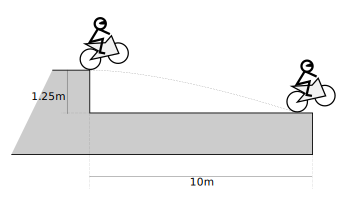
\includegraphics[width=0.8\textwidth]{moto.pdf}
\end{figure}

What was the speed at take-off?

( Soluzione a pagina \pageref{sol_p_4} )

\end{enumerate}


